The plots below show the results of our experiments. As to be expected, RMSE increases with lower preference coverage because less information in the system makes preference predictions less and less reliable. Interestingly, neither similarity measure outperforms the other for all datasets. Sometimes using the cosine similarity leads to a lower RMSE than the use of Euclidean distance, other times Euclidean distance leads to better predictions. Until a compelling answer is found to as to why one similarity measure is not consistently better than the other, we recommend that any implementers of this system run this experiment on their dataset so as to decide on which similarity measure to use to complete their market's preferences. 

We also include a plot of the same experiment on a dataset of random ordinal preferences. As per the intuition, since there are no underlying correlations between the columns, our method of using similarity measures performs exactly at the same rate as random guessing.

\begin{figure}
\begin{subfigure}{.5\textwidth}
  \centering
  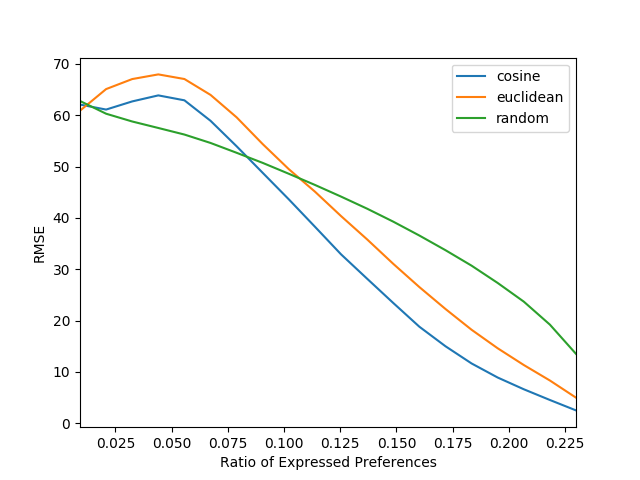
\includegraphics[width=.8\linewidth]{Sections/Plots/army.png}
  \caption{Army}
  \label{fig:army}
\end{subfigure}%
\begin{subfigure}{.5\textwidth}
  \centering
  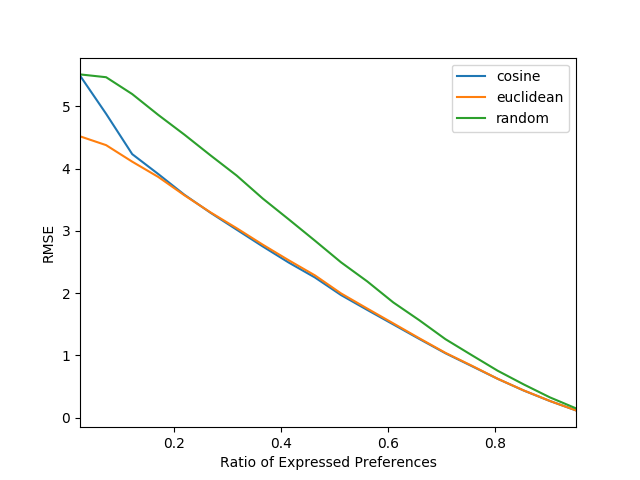
\includegraphics[width=.8\linewidth]{Sections/Plots/eod.png}
  \caption{Navy EOD}
  \label{fig:eod}
\end{subfigure}
\begin{subfigure}{.5\textwidth}
  \centering
  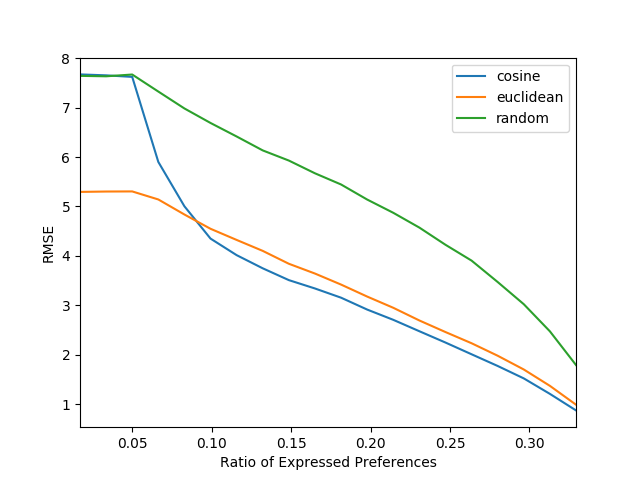
\includegraphics[width=.8\linewidth]{Sections/Plots/med_s.png}
  \caption{Navy Medical Corps Doctors}
  \label{fig:med_s}
\end{subfigure}
\begin{subfigure}{.5\textwidth}
  \centering
  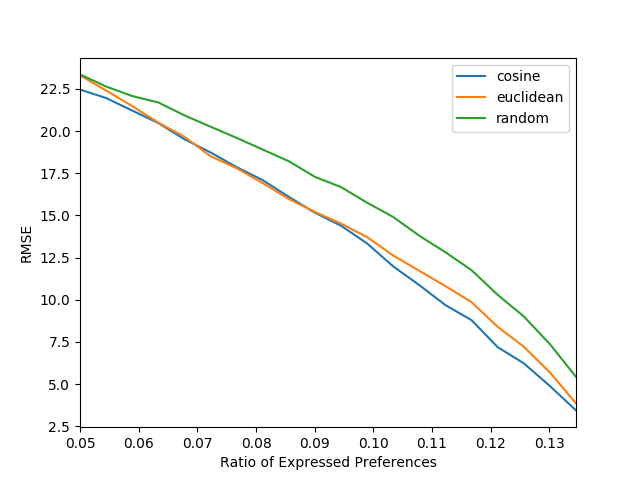
\includegraphics[width=.8\linewidth]{Sections/Plots/med_o.png}
  \caption{Navy Hospitals}
  \label{fig:med_o}
\end{subfigure}
\begin{subfigure}{.5\textwidth}
  \centering
  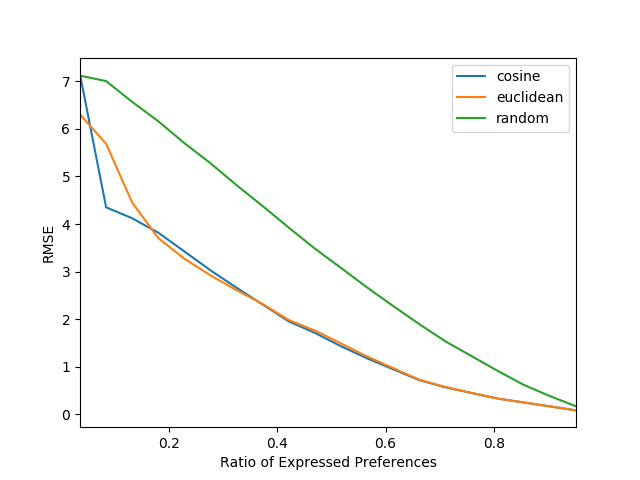
\includegraphics[width=.8\linewidth]{Sections/Plots/cw_s.png}
  \caption{Navy Cryptologic Warfare Sailors}
  \label{fig:cw_s}
\end{subfigure}
\begin{subfigure}{.5\textwidth}
  \centering
  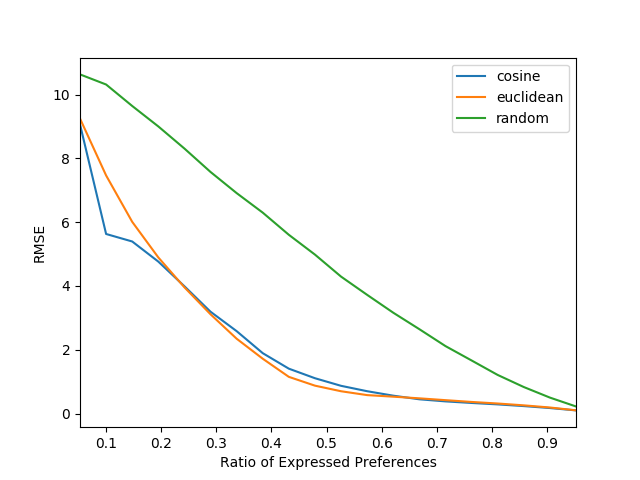
\includegraphics[width=.8\linewidth]{Sections/Plots/cw_o.png}
  \caption{Navy Cryptologic Warfare Commands}
  \label{fig:cw_o}
\end{subfigure}
\begin{subfigure}{.5\textwidth}
  \centering
  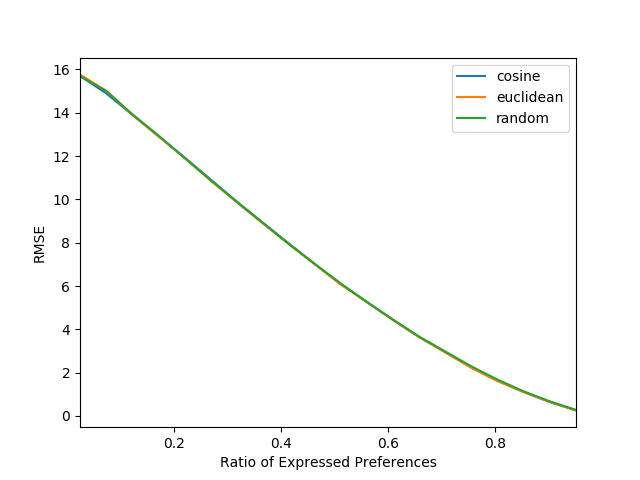
\includegraphics[width=.8\linewidth]{Sections/Plots/random.png}
  \caption{Random}
  \label{fig:random}
\end{subfigure}
\caption{Experiment Results}
\label{fig:fig}
\end{figure}

Curiously, our method is no better then random guessing, or even worse in the case of the US Army (Figure \ref{fig:army}) preference dataset, when preference coverage drops below 10\% and especially poor when below 5\%. Investigation into this phenomenon is left to future work. 

